\documentclass[main]{subfiles}

\begin{document}
% Chapter Template
\setcounter{chapter}{0}

%  Locomotion
%  A more natural approach
%   Evolutionary Algorithms
%   Chaotic systems as a source of high variability
%   Simple limiter control
\chapter{Introduction} % Main chapter title

\label{Chapter\thechapter} % Change X to a consecutive number; for referencing this chapter elsewhere, use \ref{ChapterX}

\lhead{Chapter \thechapter. \emph{Introduction}} % Change X to a consecutive number; this is for the header on each page - perhaps a shortened title

\section{Locomotion to Conquer the World}
% rev. 4

Motion is a central aspect of life for organisms on earth. %
%
When the first life evolved in oceans and other open water, most organism motion was due to environmental forces such as wind or water streams. %
%
However, with the development of more complex, multicellular organisms, self-induced motion rapidly gained importance. %
%
Different species evolved a variety of ways of locomotion such as swimming or crawling, which permitted the spread of all faunal species across oceans. %
%
With the evolution of lungs and more resistive skin, the first animals escaped water and populated the coastal regions, which surely was one of the key events of life on earth. %
%
This was however impossible with the same gaits as in water, therefore the way animals locomote had to be adapted again. %
%
Today, anthropods (including insects and spiders), recognizable by their segmented body, make up \(\unit[80]{\%}\) of all described species and have conquered every environment on earth. %
%
With the exception of some primary producers that have found a way to spread completely without self-generated motion by exploiting environmental forces to distribute seeds, organisms of higher complexity such as vertebrates depend on locomotion, usually the most complex motor behavior the organism performs \cite{bib:Grillner2000}. %
%
Locomotion is performed in different environments (e.g. air, water, ground), each with advantages and drawbacks to keep it stable. %
%
In water, fluid streams can prevent an organism from moving into one direction stably. %
%
On land, an organism faces problems with different obstacles and appropriate foot placement or switching between different gait patterns. %
%
Regardless of these problems, it seems that even very simple organisms could master the task of stable locomotion. %
%
The fundamental process of how robust, adaptive locomotion can so easily arise in many biological organisms is unfortunately largely unknown. %
%
Studies of the spinal cord suggest that a key aspect of biological, rhythmic motion is related to central pattern generators (CPG) \cite{bib:Hultborn2007}. %
%
The central pattern generator exhibits periodic and chaotic oscillations \cite{bib:Rabinovich1997} and is influenced through the aid of neuromodulation \cite{bib:Hooper2001}. %
%
They serve different rhythmic oscillations, like a function generator, for many functions in vertebrate animals, such as locomotion, breathing, peristaltic and gastric movements or other oscillatory functions. %
%
In early studies by Brown et al., it was recognized that a CPG can control simple locomotion tasks even without the need of descending motor commands from the cortex \cite{bib:Brown1911}. %
%
Additionally, in the model of the Lamprey spinal cord, stimulation of the neurons can produce fictive swimming motion, indicative of a CPG neural circuit. %
%
It was proposed that there even was a basal CPG responsible for different kinds of swimming, crawling on a surface and burrowing in the mud \cite{bib:Ayers1983}, which could be altered using neuromodulators \cite{bib:Harris-Warrick1985}. %
%
A similar CPG based mechanism was evolved to control a robotic lamprey \cite{bib:Ijspeert1999}. %
%
An extensive review of robotic CPG applications can be found by the same author \cite{bib:Ijspeert2008}. %
%

\section{A Natural Approach}
% rev. 3

Nature seems to have solved the locomotion problem of getting from point A to point B extremely easily and elegantly. %
%
Even under constraints of rough terrain and obstacles interfering with the path, a solution is nearly always found and generally does not require long path and limb trajectory planning times. %
%
It seems as if the locomotion movements arose naturally from the interaction between the legs and the ground, because we rarely see an animal look at its feet while it runs. %
%
For such gaits to be stable, the locomotion must be very robust to disturbances. %
%
Yet, engineering solutions usually rely on longer planning times and still do not reach competitive solutions in terms of robustness and adaptability to the environment. %
%
Conventionally, the need for gait adaption has to be detected, before then computing a new limb trajectory according to the chosen gait. %
%
A new approach is to design a self-adaptive system that produces a variety of periodic movements and adapts the output trajectory through the interaction with the ground. %
%
Such a system would be computationally more efficient and the produced gait more robust than conventional methods. %
%
The interaction of the body and the controller with the environment automatically constrains the motion space of the legs in order to move the leg appropriately and make the creature move forward. %
%
The sensors from the joints as well as the weight, shape, and inertia of the body parts in this system act as limiters to the feasible gait motions.

\subsection{Evolutionary Algorithms}
% rev. 2

Evolutionary algorithms mimic the general way of how evolution as a self-optimizing process finds competitive individuals able to survive on earth. %
%
The general approach is based on a population of individuals, each individual based on a genotype, an element defining the characteristics of the individual. %
%
The genotype is the blueprint of the animal and is subject to variation through mutation and crossover. %
%
The fitness functions, which model the environmental constraints that define what has to be achieved in order to be called fit, are applied to all individuals of the population to measure their fitness. %
%
If an individual is competitive with respect to the fitness functions, it has a higher chance to reproduce than a non-competitive individual. %
%
The genotypes of individuals with high fitness values are then crossed, which forms a new individual with a genotype that is a mixture of its parents' genotypes. %
%
All individuals are subject to one or multiple types of mutations, which lead to slight changes in the genotype, thereby also leading to changes in the fitness of that individual. %
%
In order to keep the size of the population constant, some of the worst performing individuals are culled. %
%
Using this process, approximately optimal solutions to NP-complete problems can be found, such as the travelling salesman problem. %
%
This is due to the features of the variation operators, crossover leading to mixtures of different solutions which are possibly better solutions than the crossed solutions, and mutation helping to produce variation and to avoid getting stuck in local minima. %
%
The evolutionary algorithm therefore follows the scheme of a general gradient descent algorithm. %
%
It must be noted that the process per se does not aim to generate better individuals and that variational operations do not necessarily lead to a better fitness of an individual. %
%
However, the population under the evolutionary process will adapt to the fitness landscape, meaning that individual solutions will converge to global minima. %
%
Very fit individuals will arise from it, not necessarily showing the same or even similar solutions, depending on the complexity of the fitness landscape. 


The locomotion task could be a challenging optimization task for evolution due to the very non-continuous nature the fitness landscape. %
%
A lack of symmetry for instance, constituting a simple change in some genome structures, can instantly make the locomotion performance drop. %
For example, a loss of one of two symmetric limbs would make it much harder to walk properly due to imbalance. %
%
Therefore, the gradient on the fitness landscape might be of little help in some areas, degrading the algorithm to random sampling. %
%
Additionally, the representation of a locomotion solution might require a large parameter space, which slows down the search for good solutions. %
%
Despite these restrictions, experiments show that the evolutionary algorithm is still applicable and finds valid solutions (see sections \ref{sec:evolved-sin-creatures} and \ref{subsec:Evolved-lim-creatures}).

\subsection{Chaotic Systems as a Source of High Variability}
% rev. 2

Chaotic systems (introduced more thoroughly in section \ref{subsec:chaotic-systems}) are the underlying model of many different physical processes such as the three-body problem in astronomy studied by Poincaré \cite{bib:Poincare1892}, population models in biology studied by Verhulst \cite{bib:Verhulst1838}, weather models in meteorology studied by Lorenz \cite{bib:Lorenz1963} and many other models from different fields. %
%
Before the beginning of chaos theory dated back to the 19th century, it was thought that approximate knowledge about the initial state of a deterministic system was sufficient to approximate knowledge about the future. %
%
In natural sciences, the exact knowledge of a real-world state of a system is impossible, as the real-valued nature of a natural, continuous system state has infinite precision. %
%
However, an experiment can only reveal a limited-precision state of the system. %
%
Chaos theory showed that a small variation of the initial conditions can cause a large variation in the future state, as already Poincaré put it when studying the three-body problem. %
%
The former belief that all deterministic systems can be perfectly predicted using approximate knowledge turned out false for most systems \cite{bib:Motter2013}. %
%
Instead it was found that such unpredictable systems had to be studied much more in-depth to understand; when different initial conditions converge to the same solutions, and what conditions lead to a variety of different outcomes. %
%
It is the property leading to the unpredictability, namely the sensitivity to the initial conditions, that can be used to produce a high variability of trajectories. %
%
In a chaotic system, the trajectories are guided by an infinite amount of unstable periodic orbits (UPOs), that, in interaction with each other, lead to the variability of trajectories. %
%
Using a chaotic system and a chaos control method together with an evolutionary algorithm, the evolutionary algorithm could tune the system's output to show a desired solution trajectory to simplify the emergence of robust locomotion. %
%
As it turns out, simple limiters, introduced in the next section, are a very natural way of influencing chaotic systems. %
%
Through their innate coupling with the chaotic system, because they express limitations in the state space in the same 'language' as the system and are hence elegant by simplicity, simple limiters could be the key to control the system into different trajectories for periodic and chaotic movement. %

\subsection{Simple Limiter Control}
% rev. 1

Simple limiter control, first introduced in the paper by Ned J. Corron et al. in 2000 \cite{bib:Corron2000}, is different from other preceding chaos control strategies. %
%
The OGY method described by Ott, Grebogi and Yorke \cite{bib:Ott1990}, one of the first chaos control methods at hand, states that small, wisely chosen perturbations applied to the system can stabilize a particular UPO. %
%
The perturbation must be applied once per cycle, but the chaotic system must be intensively studied through an appropriate Poincaré section to understand what the precise perturbation must be. %
%
The time to measure, generate and apply a control signal, called the latency of the OGY method, is another limitation that allows only for a certain range of frequency control. %
%
The simple limiter control method is much more simple. A limiter expresses a limitation in the state space of the chaotic system and thereby suppresses certain periodic orbits. %
%
%
Interestingly, however, the remaining reachable periodic orbits are being stabilized. %
%
The seemingly unpredictable trajectory always deterministically switches at the same point to the same periodic orbits in the phase space. %
%
Using the simple limiter, the switching can be prevented at some specified point and leave the system state no other choice than to stay on its current orbit and to repeat its trajectory, and hence the state is stabilized on a trajectory of a certain periodicity. %
%
In 2001, Wagner and Stoop showed that the optimal simple limiter control ranges for different limit cycles can be found using the derivative of the system \cite{bib:Wagner2001}. %
%
In a natural system such as the actuated leg joint, this limiter can be much more subliminal, be it the weight or dimensions of the body parts or the limits, damping or friction of the joints, or even the fact that two physical objects can not interpenetrate each other. %
%

\subsection{Experiment Outline}

\todo[inline]{Add a chart depicting all performed experiments}
\begin{figure}[H]
\centering
\begin{tikzpicture}
% classes
\pgfdeclarelayer{background}
\pgfdeclarelayer{foreground}
\pgfsetlayers{background,main,foreground}
\tikzstyle{bigbox} = [draw=black!80, thick, fill=black!5, rounded corners, rectangle]
\tikzstyle{box} = [minimum size=0.6cm,draw=black!80, thick,rounded corners, rectangle, fill=black!20]

\node(experiments) at (0,0){\Large\underline{Experiments}};

%###############################################
% Mathematica experiments
%###############################################
\node(mathematica-experiments)[below right =0.3cm and -3cm of experiments]{\underline{Mathematica experiments}};
\node(mathematica-image)[below=0.5cm of mathematica-experiments]{
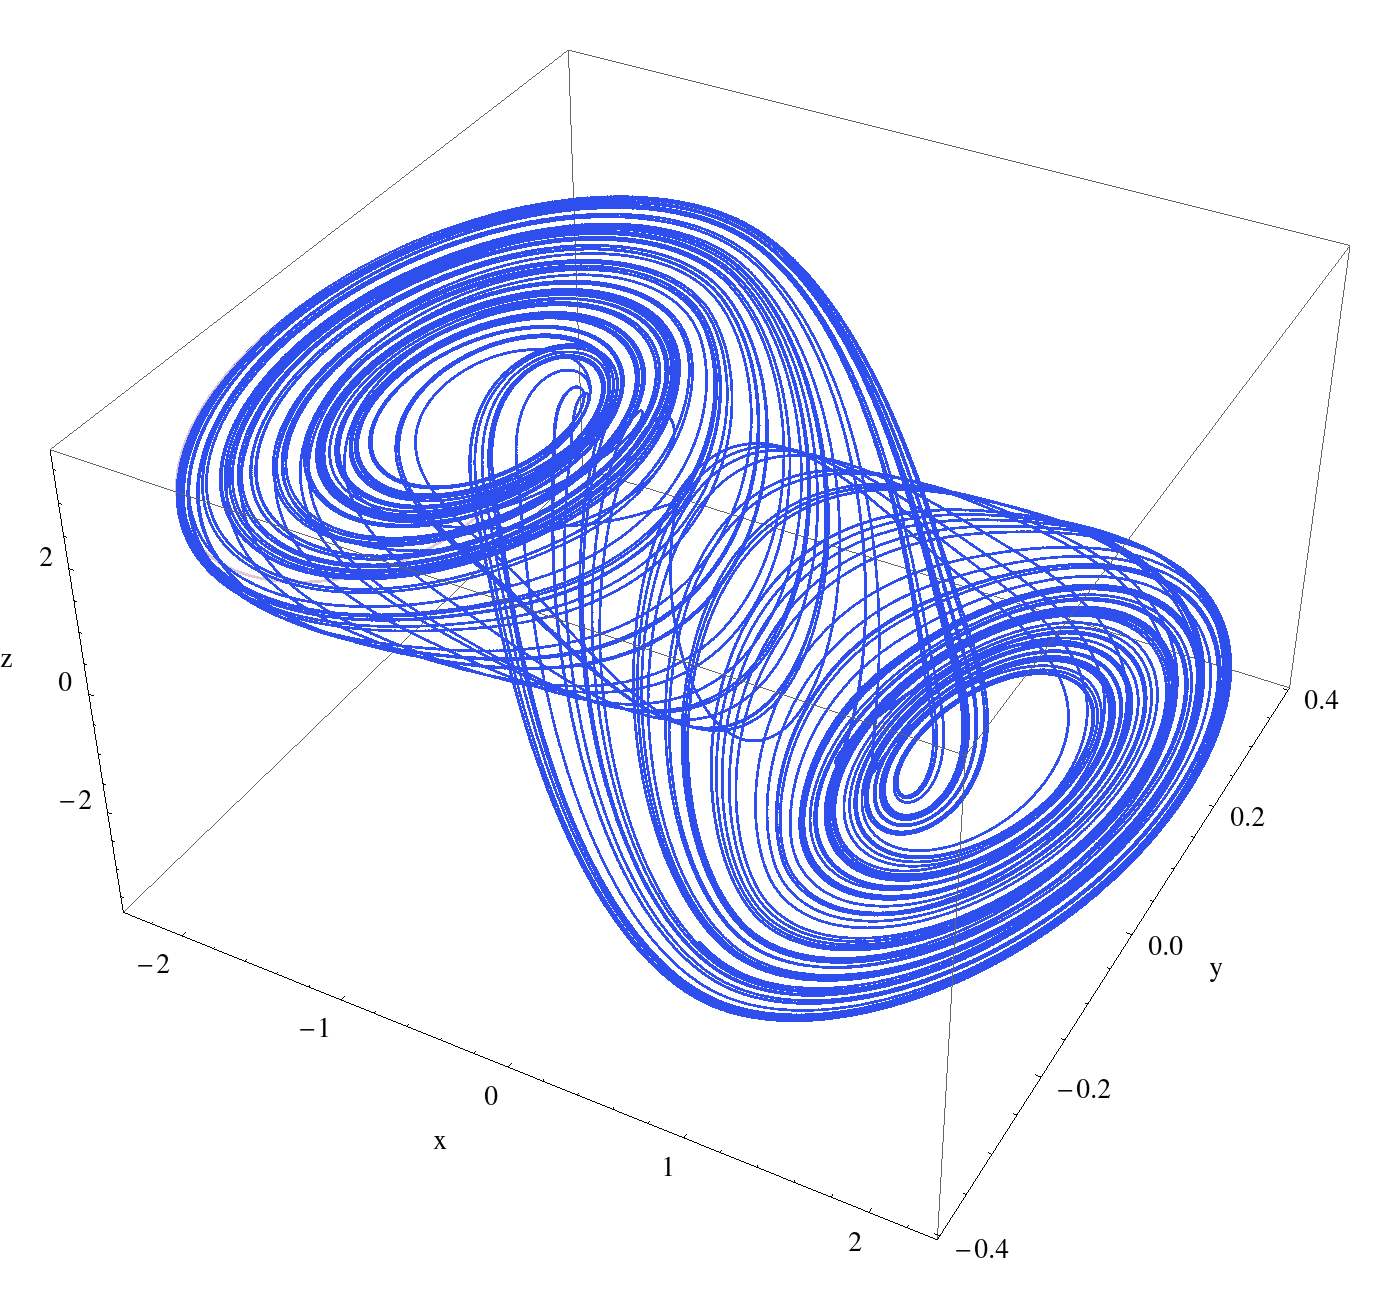
\includegraphics[scale=0.04]{Pictures/controllers/chua-circuit/Unlimited-chua-circuit.png}
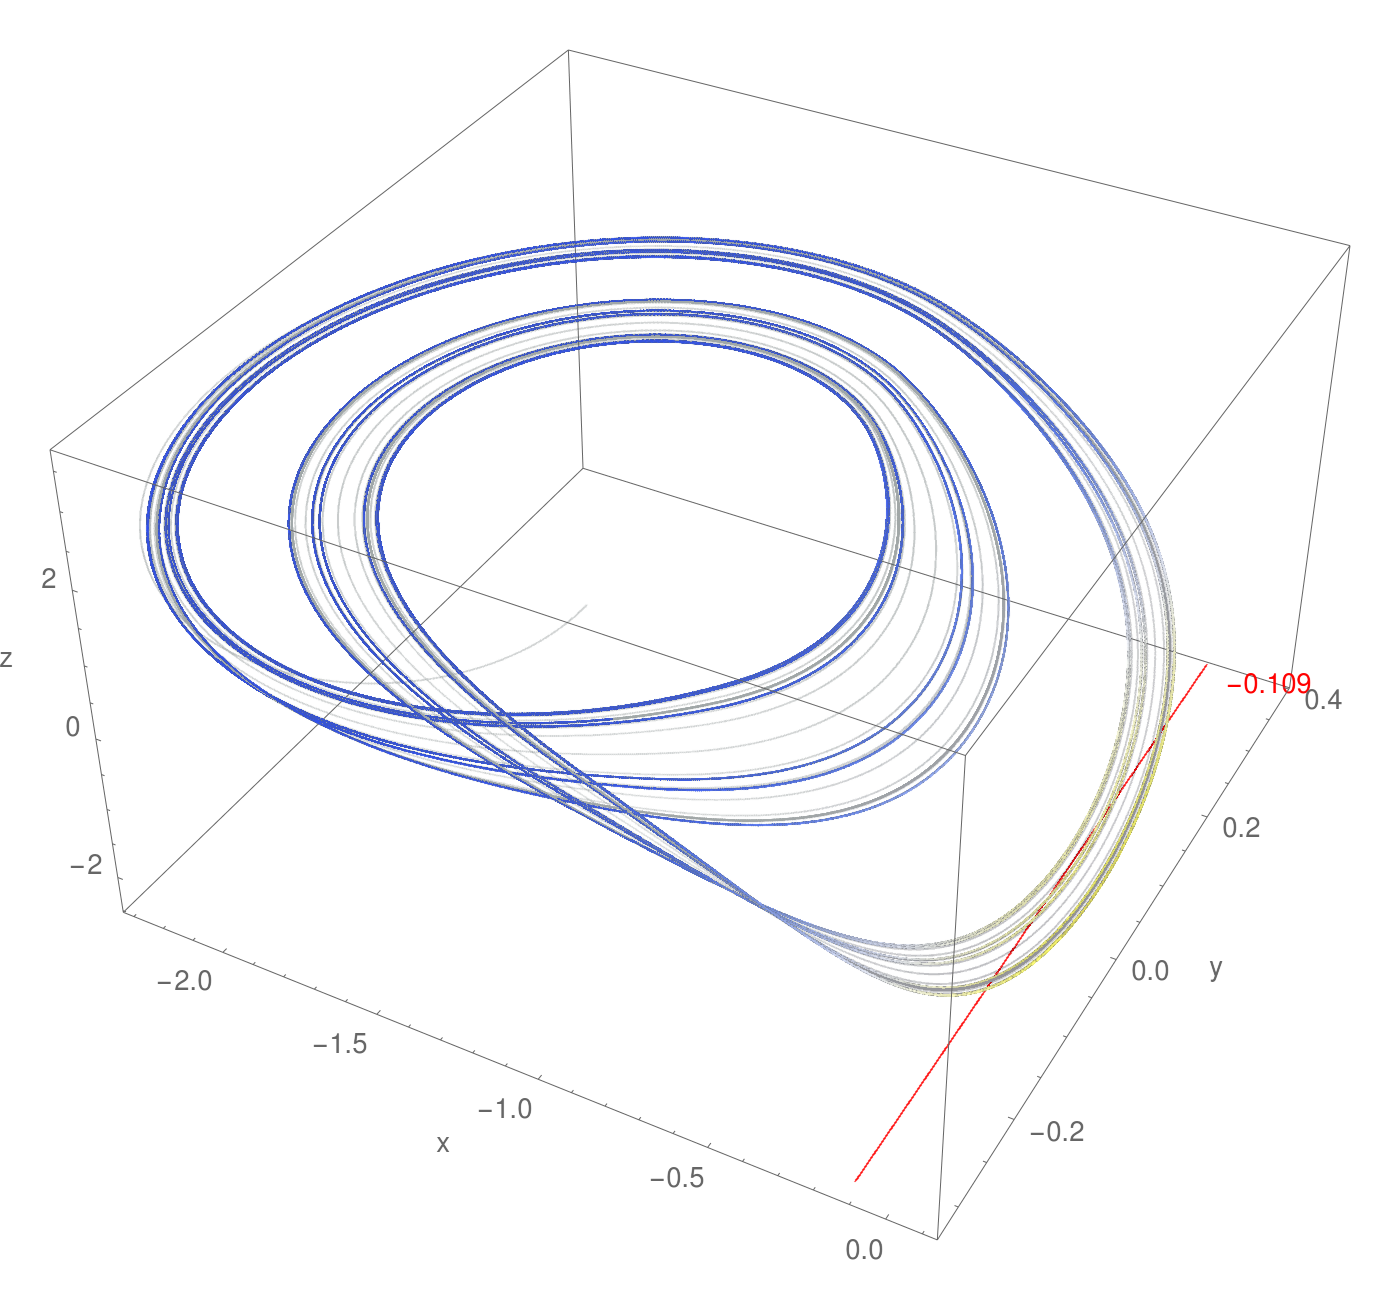
\includegraphics[scale=0.04]{Pictures/controllers/chua-circuit/Limited-chua-circuit-x-softness-0-5--0-109-convergence.png}
};
\node(mathematica-text)[below=0.6cm of mathematica-image,align=left]{
\scriptsize{\begin{varwidth}{4cm}Simple limiter experiments on the Chua circuit\end{varwidth}}
 };

%###############################################
% Chaotic controller experiments
%###############################################
\node(chaotic-controller-experiments)[right=0.7cm of mathematica-experiments]{\underline{Chaotic controller experiments}};
\node(chaotic-controller-image)[below=0.1cm of chaotic-controller-experiments]{
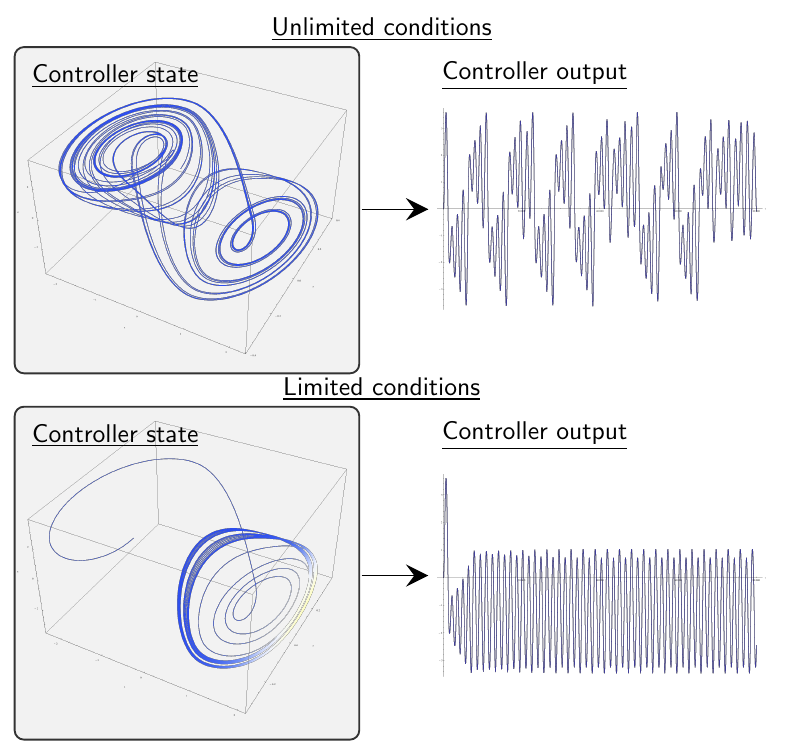
\includegraphics[scale=0.1]{Pictures/introduction/chaotic-controller.png}
};
\node(chaotic-controller-text)[below=0.1cm of chaotic-controller-image,align=left]{
\scriptsize{\begin{varwidth}{4cm}Experiments related to the indirectly limited chaotic controller\end{varwidth}}
 };
 
%###############################################
% Sinusoidal controller experiment
%###############################################
\node(sinusoidal-controller-experiments)[right=0.7cm of chaotic-controller-experiments]{\underline{Sinusoidal controller experiments}};
\node(sinusoidal-controller-image1)[below=0.1cm of sinusoidal-controller-experiments]{
\includegraphics[scale=0.2]{results/evolved-creatures/sine/jumper1/jumper1-animation.png}
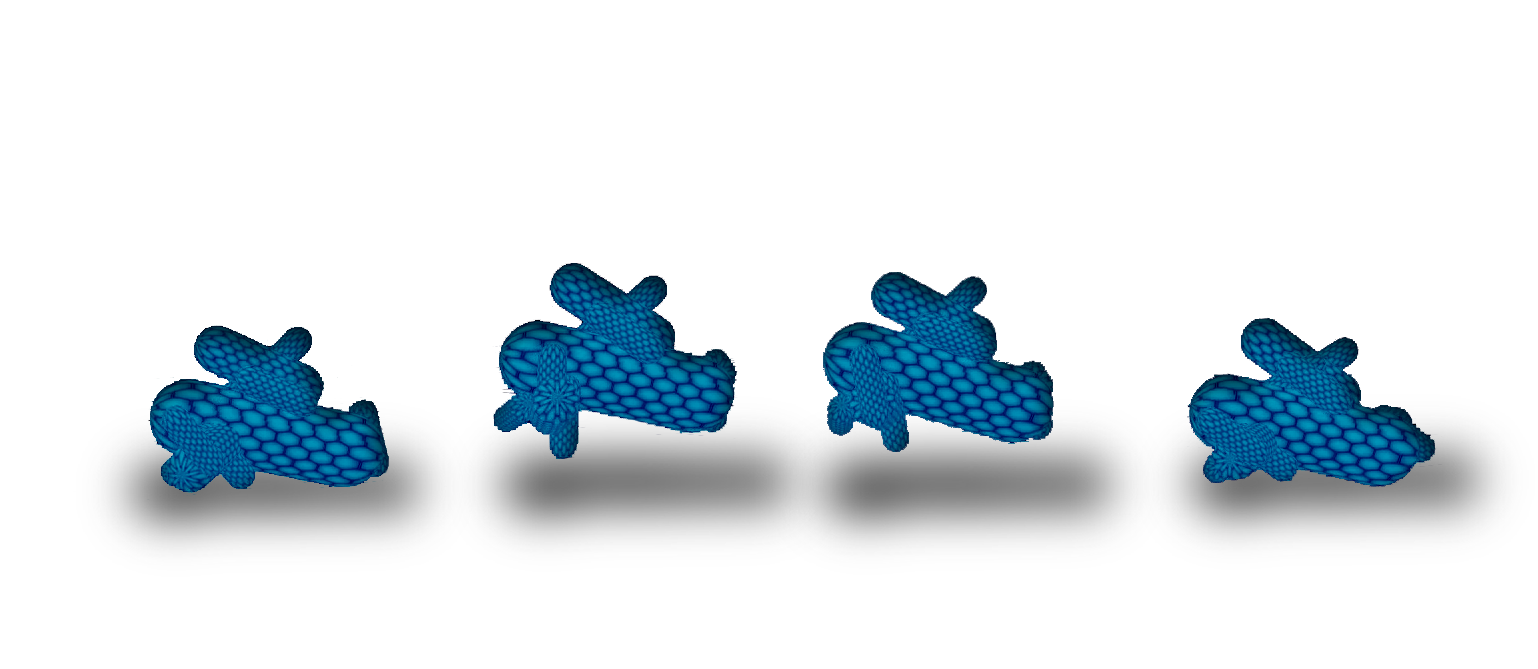
\includegraphics[scale=0.2]{results/evolved-creatures/sine/jumper2/jumper2-animation.png}
};
\node(sinusoidal-controller-image2)[below=0cm of sinusoidal-controller-image1]{
\includegraphics[scale=0.2]{results/evolved-creatures/sine/walker1/walker1-animation.png}
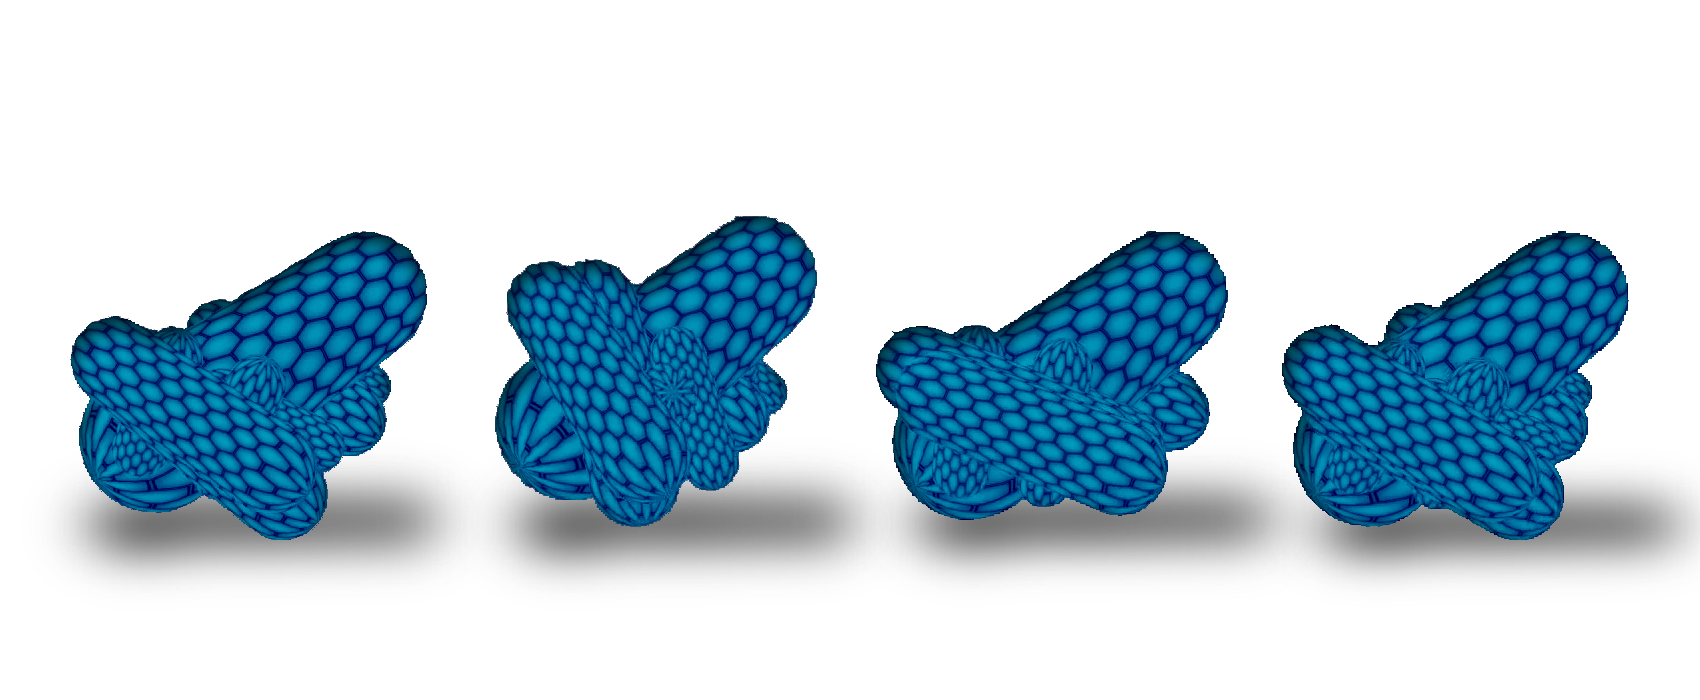
\includegraphics[scale=0.2]{results/evolved-creatures/sine/walker2/walker2-animation.png}
};
\node(sinusoidal-controller-text)[below=0.1cm of sinusoidal-controller-image2,align=left]{
\scriptsize{\begin{varwidth}{4cm}Evolving creatures using the sinusoidal controller\end{varwidth}}
 };

%###############################################
% ## Indirectly limited chaotic controller experiments
%###############################################
\node(indirect-limiter-controller-experiments)[below=1cm of chaotic-controller-text]{\scriptsize\underline{Indirectly limited controller experiments}};
\node(indirect-limiter-controller-image)[below=0.1cm of indirect-limiter-controller-experiments]{
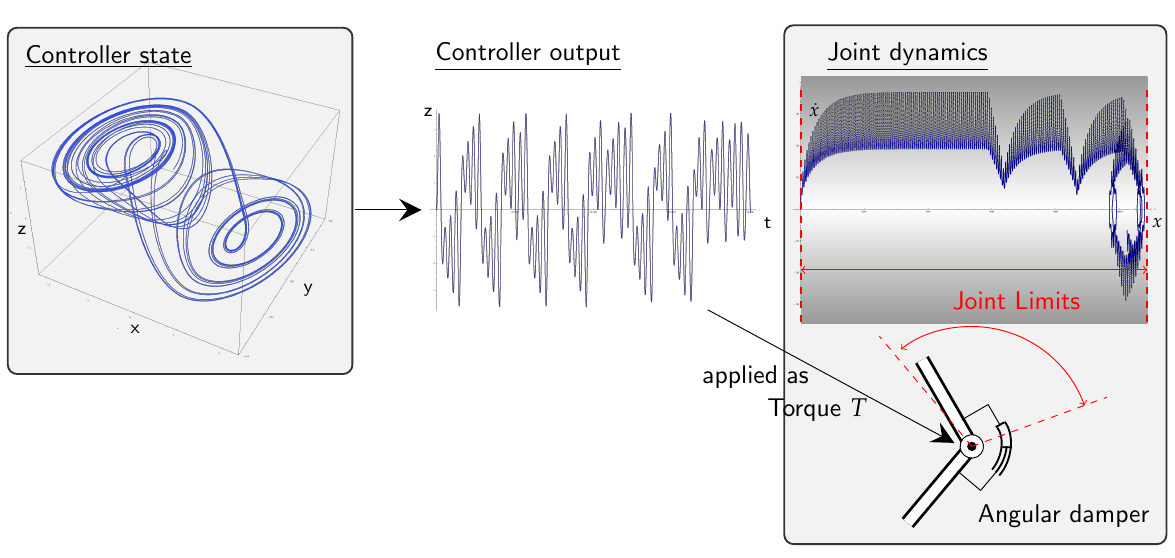
\includegraphics[scale=0.13]{Pictures/introduction/indirectly-limited-controller.png}
};
\node(indirect-limiter-controller-text)[below=0.1cm of indirect-limiter-controller-image,align=left]{
\scriptsize{\begin{varwidth}{4cm}Experiments using the indirectly limited chaotic controller\end{varwidth}}
 };

%###############################################
% ### Evolution experiments
%###############################################
\node(il-evolution-experiments)[below=0.5cm of indirect-limiter-controller-text]{\scriptsize\underline{Evolved organism experiments}};
\node(il-evolution-image)[below=0.1cm of il-evolution-experiments]{
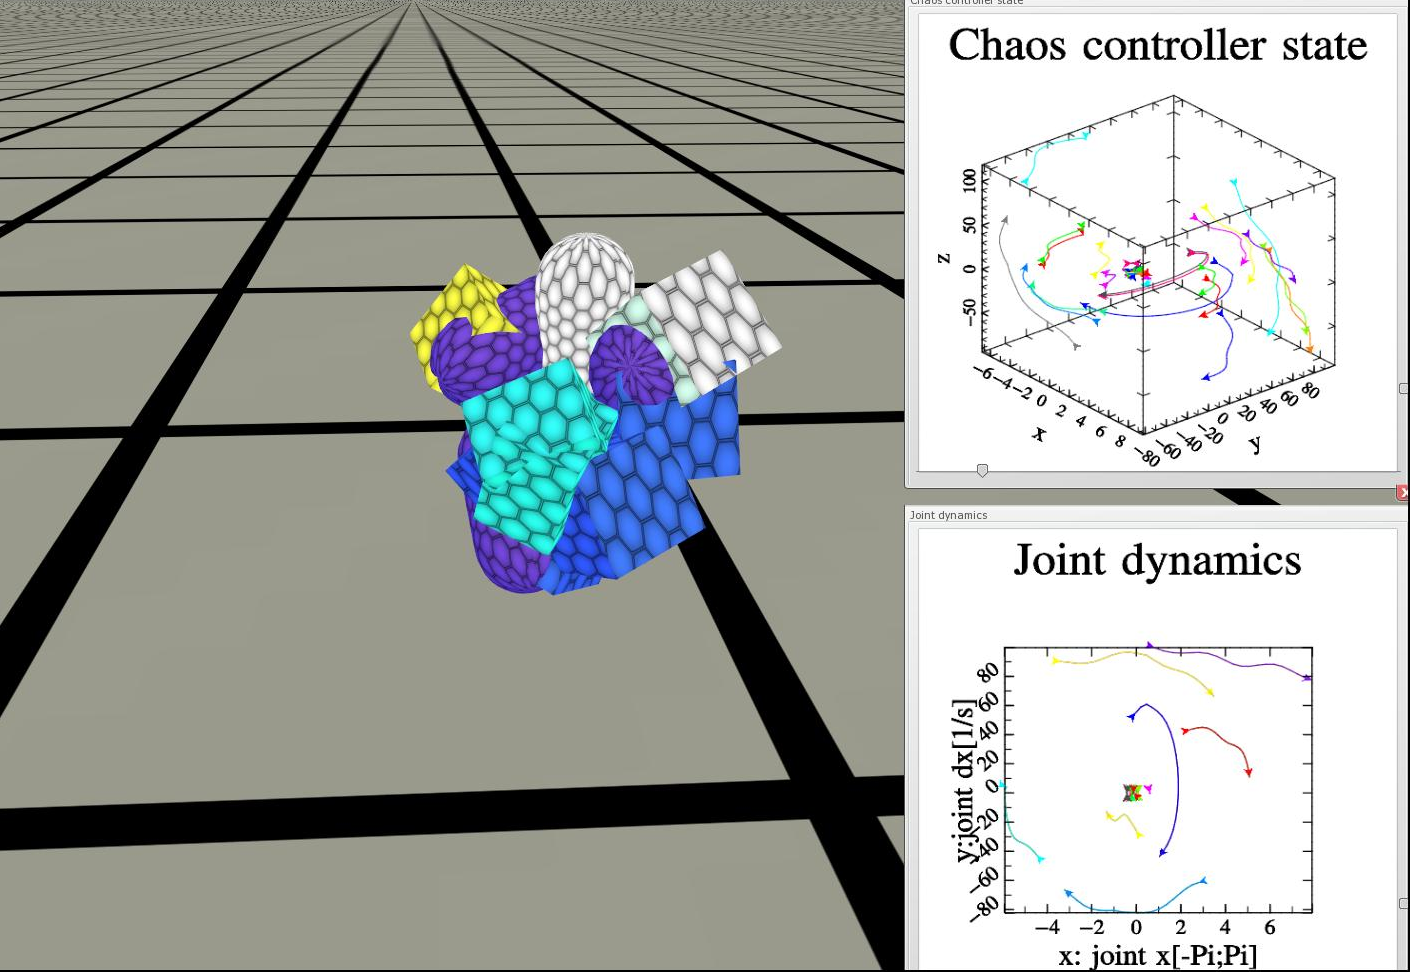
\includegraphics[scale=0.1]{Pictures/introduction/indirectly-limited-evolution.png}
};
\node(il-evolution-text)[below=0.1cm of il-evolution-image,align=left]{
\scriptsize{\begin{varwidth}{4cm}Evolving creatures using indirectly limited, chaotic controllers\end{varwidth}}
 };
 
%###############################################
% ## Model leg experiments
%###############################################
\node(model-leg-experiments)[left=1.7cm of indirect-limiter-controller-experiments]{\scriptsize\underline{Model leg experiments}};
\node(model-leg-image)[below=0.1cm of model-leg-experiments]{
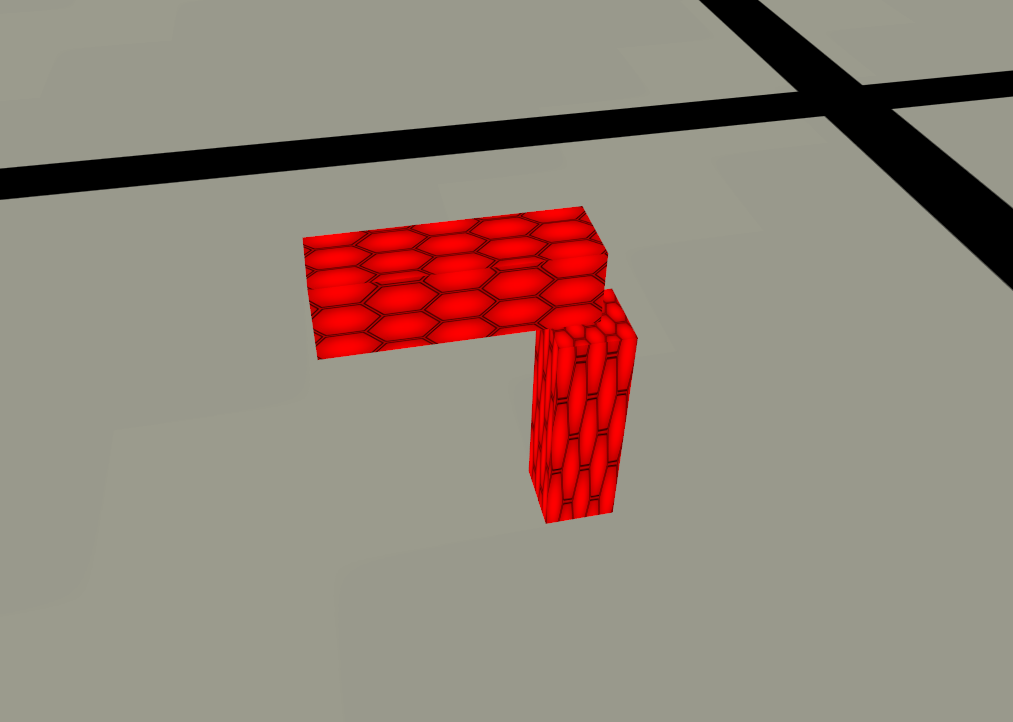
\includegraphics[scale=0.13]{Pictures/model-organisms/Model-leg2.png}
};
\node(model-leg-graph-image)[below=0cm of model-leg-image]{
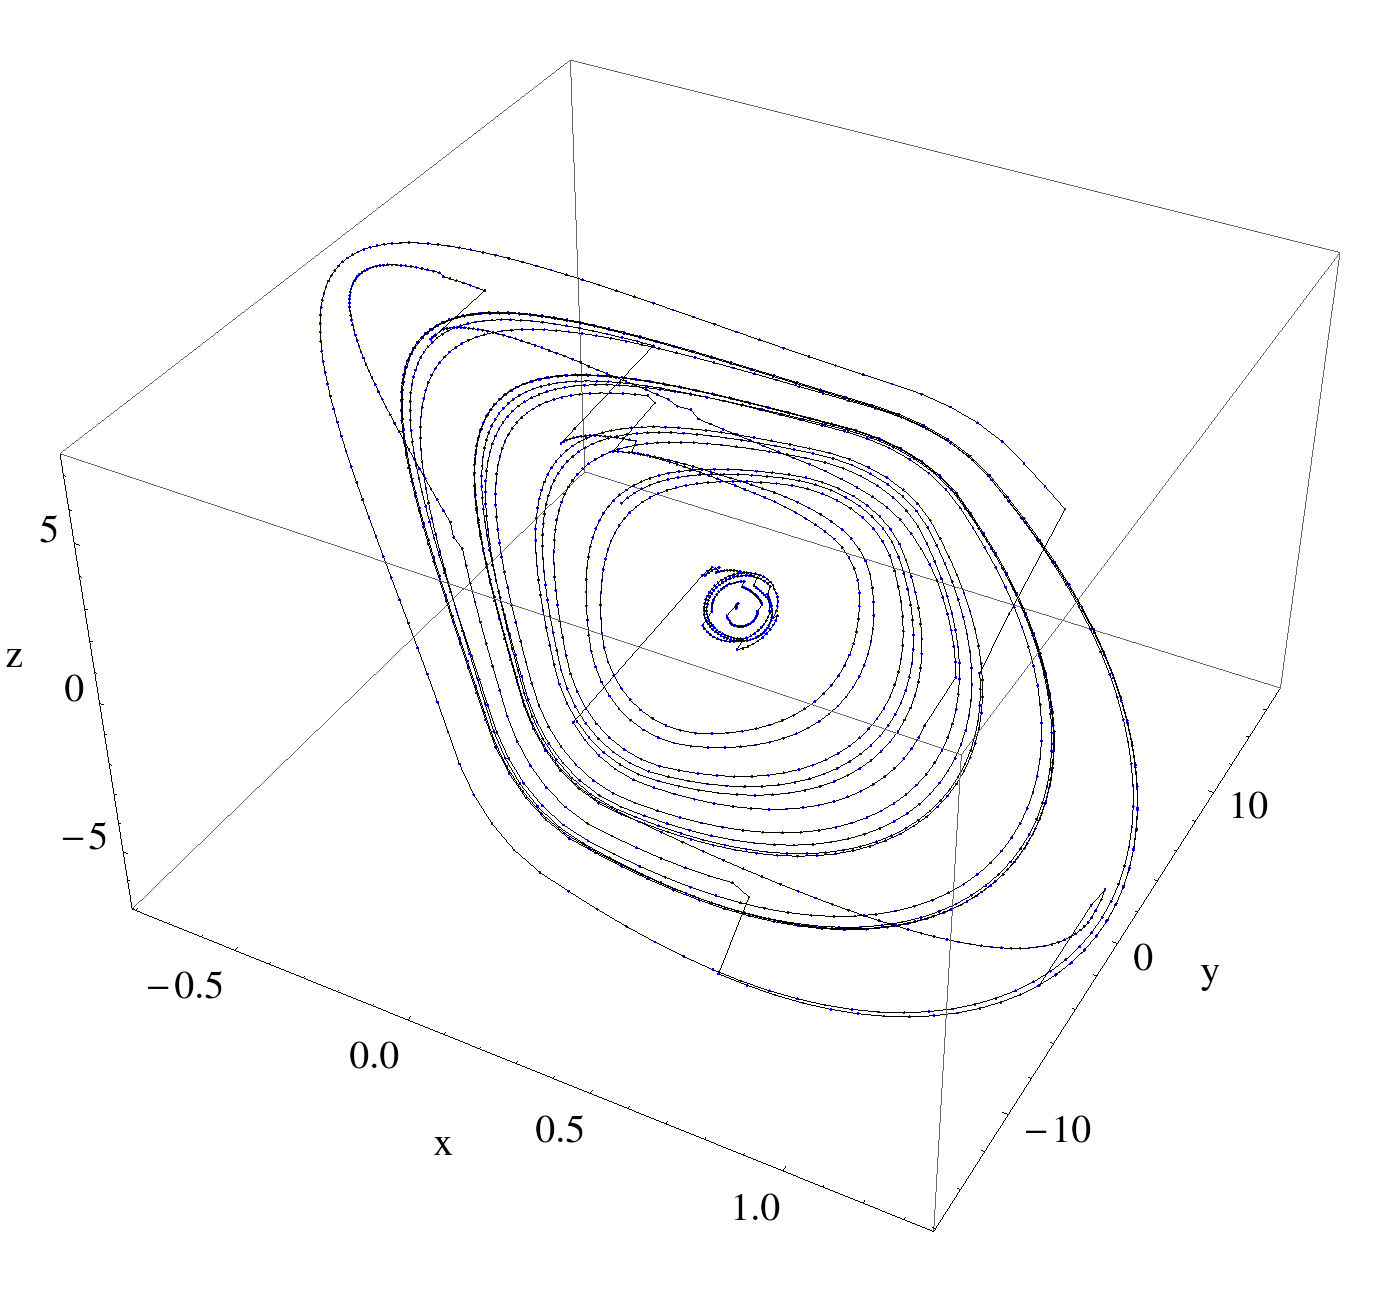
\includegraphics[scale=0.1]{Pictures/model-organisms/model-leg/Modelleg-1g-100s-friction11-force2-damping0-xyz.png}
};
\node(model-leg-text)[below=0.1cm of model-leg-graph-image,align=left]{
\scriptsize{\begin{varwidth}{4cm}Parameter exploration on the model leg\end{varwidth}}
 };



%###############################################
% ## Directly limited chaotic controller experiments
%###############################################
\node(direct-limiter-controller-experiments)[right=1.2cm of indirect-limiter-controller-experiments]{\scriptsize\underline{Directly limited controller experiments}};
\node(direct-limiter-controller-image)[below=0.1cm of direct-limiter-controller-experiments]{
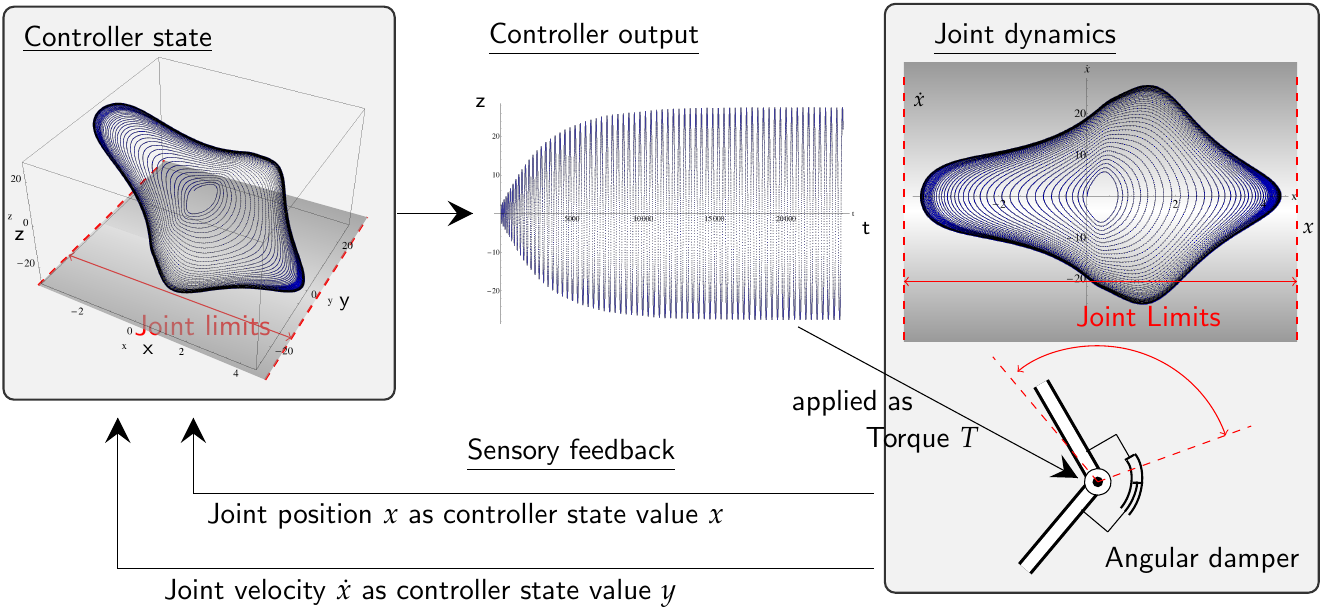
\includegraphics[scale=0.13]{Pictures/introduction/directly-limited-controller.png}
};
\node(direct-limiter-controller-text)[below=0.1cm of direct-limiter-controller-image,align=left]{
\scriptsize{\begin{varwidth}{4cm}Experiments using the directly limited, chaotic controller\end{varwidth}}
 };

%###############################################
%## Evolution experiments
%###############################################
\node(dl-evolution-experiments)[below right =0.5cm and -4.1cm of direct-limiter-controller-text]{\scriptsize\underline{Evolved organism experiments}};
\node(dl-evolution-experiments-image1)[below=0.1cm of dl-evolution-experiments]{
\includegraphics[scale=0.11]{results/evolved-creatures/chaotic/jumper1/jumper1-animation.png}
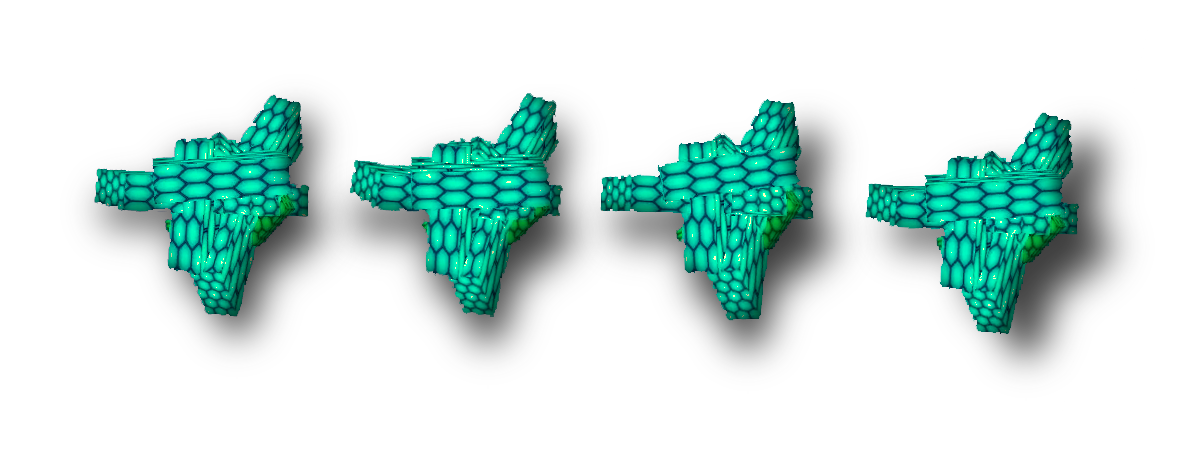
\includegraphics[scale=0.26]{results/evolved-creatures/chaotic/crawler1/crawler1-animation.png}
};
\node(dl-evolution-experiments-image2)[below=0cm of dl-evolution-experiments-image1]{
\includegraphics[scale=0.16]{results/evolved-creatures/chaotic/walker1/walker1-animation.png}
};
\node(dl-evolution-text)[below=0.1cm of dl-evolution-experiments-image2,align=left]{
\scriptsize{\begin{varwidth}{4cm}Evolving creatures using directly limited chaotic controllers\end{varwidth}}
 };

\begin{pgfonlayer}{background}
  \node(main-big-box)[bigbox] [fit = (experiments) (mathematica-experiments) (mathematica-image)(mathematica-text)
				     (sinusoidal-controller-experiments) (sinusoidal-controller-image1) (sinusoidal-controller-image2) (sinusoidal-controller-text)
				     (chaotic-controller-experiments) (chaotic-controller-image)(chaotic-controller-text)
				     (model-leg-experiments) (model-leg-image) (model-leg-graph-image) (model-leg-text)
				     (indirect-limiter-controller-experiments) (indirect-limiter-controller-image)(indirect-limiter-controller-text)
				     (il-evolution-experiments) (il-evolution-image)(il-evolution-text)
				     (direct-limiter-controller-experiments) (direct-limiter-controller-image) (direct-limiter-controller-text)
				     (dl-evolution-experiments)  (dl-evolution-experiments-image1) (dl-evolution-experiments-image2)(dl-evolution-text),inner sep=15pt,outer sep=15pt] {};
  
  \node(chaotic-controller-experiments-box)[bigbox][fit = (model-leg-experiments) (model-leg-image) (model-leg-graph-image) (model-leg-text)
  (indirect-limiter-controller-experiments) (indirect-limiter-controller-image)(indirect-limiter-controller-text)
  (il-evolution-experiments) (il-evolution-image)(il-evolution-text)
  (direct-limiter-controller-experiments) (dl-evolution-experiments-image1) (dl-evolution-experiments-image2)(direct-limiter-controller-text)
  (dl-evolution-experiments)  (dl-evolution-experiments-image1) (dl-evolution-experiments-image2)(dl-evolution-text),inner sep=10pt]{};
  
  \node(mathematica-box)[box][fit = (mathematica-experiments) (mathematica-image)(mathematica-text)]{};
  \node(sinusoidal-box)[box][fit = (sinusoidal-controller-experiments) (sinusoidal-controller-image1) (sinusoidal-controller-image2) (sinusoidal-controller-text)]{};
  \node(chaotic-box)[box][fit = (chaotic-controller-experiments) (chaotic-controller-image)(chaotic-controller-text)]{};
  \node(model-leg-box)[box][fit = (model-leg-experiments) (model-leg-image) (model-leg-graph-image) (model-leg-text)]{};
  \node(indirect-controller-box)[box][fit = (indirect-limiter-controller-experiments) (indirect-limiter-controller-image)(indirect-limiter-controller-text)]{};
  \node(il-evolution-box)[box][fit = (il-evolution-experiments) (il-evolution-image)(il-evolution-text)]{};
  \node(direct-controller-box)[box][fit = (direct-limiter-controller-experiments)  (direct-limiter-controller-image) (direct-limiter-controller-text)]{};
  \node(dl-evolution-box)[box][fit = (dl-evolution-experiments)  (dl-evolution-experiments-image1) (dl-evolution-experiments-image2)(dl-evolution-text)]{};
  
\end{pgfonlayer}

\draw (chaotic-box.south west) -- (chaotic-controller-experiments-box.north west);
\draw (chaotic-box.south east) -- (chaotic-controller-experiments-box.north east);
 
\fill [path fading=south,black!10] (chaotic-box.south west) to (chaotic-box.south east) to (chaotic-controller-experiments-box.north east) to (chaotic-controller-experiments-box.north west) to (chaotic-box.south west);




\end{tikzpicture}


\caption[The experiments chart]{The chart of experiments performed for this thesis.}
\label{figure:experiments-chart}
\end{figure}

The goal of this thesis is to use evolutionary algorithms and the above mentioned, chaotic control system to evolve creatures in a rigid-body physics engine to find example creatures showing basic locomotion abilities emerge in the interaction with the ground. %

Therefore, a simulator is developed to evolve artificial creatures using a specially tailored type of genome to co-evolve the individual's controller and morphology. %

In a first evolution, the creature's movement is controlled by an engineered controller emitting sinusoidal leg movement signals, so that each joint degree of freedom moves according to the sinusoid's parameters of amplitude, frequency and offset. %

After successful evolution of locomoting creatures, an example chaotic system is chosen and a simple limiter is applied to it to observe the influence of different simple limiter configurations. %

Then, creatures are evolved being driven by chaotic leg movement controllers using the previously chaotic system to exert joint torques. %

In case the controller does
\end{document}